%% $Id: thesis.tex,v 1.16 2004/09/01 14:37:00 yahave Exp $

%%%%%%%%%%%%%%%%%%%%%%%%%%%%%%%%%%%%%%%%%%%%%%%%%%%%%%%%%%%%%%%%%%%%%%
%%
%%  UT-THESIS.TEX
%%  Copyright (c) 1999 by Francois Pitt
%%  Last Update: 1999 May 13
%%
%%%%%%%%%%%%%%%%%%%%%%%%%%%%%%%%%%%%%%%%%%%%%%%%%%%%%%%%%%%%%%%%%%%%%%
%%
%%  This file is distributed in the hope that it will be useful but
%%  without any warranty (without even the implied warranty of
%%  fitness for a particular purpose).  For a description of this
%%  file's purpose, and instructions on its use, see below.
%%
%%  Feel free to copy and redistribute this file, as long as this
%%  copyright notice remains intact and this file is distributed
%%  along with the companion file `ut-thesis.cls'.
%%
%%  (Thanks to Robert Bernecky for his suggestions on improving the
%%  usefulness and readability of this file.)
%%
%%  Send all bugs, questions, comments, suggestions, etc. to the
%%  author, at <fpitt@cs.utoronto.ca>.
%%
%%%%%%%%%%%%%%%%%%%%%%%%%%%%%%%%%%%%%%%%%%%%%%%%%%%%%%%%%%%%%%%%%%%%%%
%%
%%  Skeleton LaTeX2e file for the preparation of theses at UofT;
%%  conforms to the School of Graduate Studies' guidelines of 07/97.
%%  To be used in conjunction with class file `ut-thesis.cls', whose
%%  features it illustrates.
%%
%%  To comment out parts of a file, use the macro \ignore{...}
%%  around the entire block of text you want to ignore.
%%
%%  To explicitly set the pagestyle of any inserted blank page when
%%  \cleardoublepage occurs, use one of \clearemptydoublepage or
%%  \clearplaindoublepage instead.
%%
%%  For single-spaced quotes or quotations, use the `longquote' and
%%  `longquotation' environments.  For single-spaced, 1 1/2-spaced,
%%  or double-spaced paragraphs, use one of the environments
%%  `singlespaced', `oneandahalfspaced', or `doublespaced'.  More
%%  generally, for paragraphs with a line spacing of `n', use
%%  `\begin{newspacing}{n}...\end{newspacing}'.
%%
%%  All other environments, commands, and options provided by the
%%  `ut-thesis' class will be described below, at the point where
%%  they should appear in the document.
%%
%%  See the companion file `ut-thesis.cls' for more details.
%%
%%%%%%%%%%%%%%%%%%%%%%%%%%%%%%%%%%%%%%%%%%%%%%%%%%%%%%%%%%%%%%%%%%%%%%


%%%%%%%%%%%%         PREAMBLE         %%%%%%%%%%%%

%% Default settings format a final copy (12pt font, single-sided,
%% double-spaced, normal margins, single-spaced notes).  For a rough
%% copy (10pt font, double-sided, double-spaced, normal margins, with
%% the word "DRAFT" printed at each corner of every page), use the
%% `draft' option.  The default line spacing can be changed with one
%% of the following options: `singlespaced', `oneandahalfspaced', or
%% `doublespaced'.  The notes are always single-spaced by default, but
%% can be made to have the same spacing as the rest of the document by
%% using the option `spacednotes'.  The size of the margins can be
%% changed with one of the following options: `narrowmargins' (1 1/4"
%% left, 3/4" others), `normalmargins' (1 1/4" left, 1" others),
%% `widemargins' (1 1/4" all), `extrawidemargins' (1 1/2" all).  Any
%% other standard option for the `report' document class can be used
%% to override the default or draft settings.

%% ***   Add any desired options.   ***
%%\documentclass{ut-thesis}

%% production
\newcommand{\myDocOptions}{11pt,twoside,openright,oneandahalfspaced,normalmargins}
\documentclass[pdftex,\myDocOptions]{ut-thesis}


\newcommand{\myTitle}{Chopped Symbolic Execution}
\newcommand{\myAuthor}{David Trabish}


%% ***   Add \usepackage declarations here.   ***

\pdfoutput=1
\usepackage[pdftex,bookmarks=true,colorlinks=true, pdfstartview=FitV, linkcolor=blue,
         citecolor=blue, urlcolor=blue,plainpages=false]{hyperref}
\usepackage[pdftex]{graphicx}
\pdfinfo{
    /Title    (\myTitle)
    /Author   (\myAuthor)
    /Keywords (Symbolic Exwcution, Static Analysis, Compilers, Program Analysis)
    /Keywords ()
}


\usepackage{amsthm}
\usepackage{amsfonts}
\usepackage{amssymb}
\usepackage{alltt}
\usepackage{times}
\usepackage{fancyvrb}
\usepackage{import}
\usepackage{epsfig}
\usepackage{stmaryrd}
\usepackage{graphicx}
\usepackage{enumerate}
\usepackage[usenames]{color}
\usepackage{makeidx}
\usepackage[caption=false]{subfig}
\usepackage{longtable}
\usepackage{floatrow}
\usepackage{tikz}

% customized packages

\usepackage{booktabs} % For formal tables

\usepackage{amsmath}
\usepackage{MnSymbol}
%\usepackage{amssymb}
%\usepackage{stmaryrd}
\usepackage{array}
\usepackage{listings}
\usepackage[shadow]{todonotes}
\usepackage{xspace}
\usepackage{paralist}
\let\labelindent\relax
\usepackage{enumitem}
\usepackage{multirow}
\usepackage{xcolor,colortbl}
\usepackage{flushend}
\usepackage{makecell}
\usepackage{arydshln}
\usepackage{mdframed}
\usepackage{flushend}
%\usepackage[utf8]{inputenc}
\usepackage[T1]{fontenc}
\usepackage{microtype}
\usepackage{algpseudocode}
\usepackage{algorithm}
\usepackage{alltt}
%\usepackage{amsmath,MnSymbol}% ,stmaryrd,amssymb,amsfonts,MnSymbol}
\usepackage{extarrows}
\usepackage{stackrel}
\usepackage{stfloats} % Fixes problem with latex2e figures
\usepackage{makecell}
\usepackage{graphicx}
\usepackage{adjustbox}
\usepackage{verbatim}

\usepackage{datetime}
\usepackage{todonotes}

\usepackage{cleveref} % Must be included last


\lstset{language=C++,
    numberstyle=\footnotesize,
    numbers=left,
    numbersep=5pt,
    numberblanklines=true,
    captionpos=b,
    basicstyle=\footnotesize\ttfamily,
    columns=flexible,
    xleftmargin=16pt,
    frame=none,
    tabsize=2,
    escapeinside={/*@}{@*/},
}

\makeatletter
\@addtoreset{example}{chapter}
\@addtoreset{lemma}{chapter}
\@addtoreset{theorem}{chapter}
\makeatother

\theoremstyle{definition}
\newtheorem{example}{Example}[section]
\newtheorem{lemma}{Lemma}[section]
\newtheorem{theorem}{Theorem}[section]
%% The line spacing of the document should be specified using one of
%% the document options given above, but if you need a line spacing
%% that is not provided by the options, you can override the default
%% line spacing for the entire document with the command
%%   `\linespacing{...}'.
%% Note that in order to get the correct appearance, the argument to
%% `\linespacing' must be equal to 1/3 + 2/3 times the desired line
%% spacing (for example, single-spaced = \linespacing{1},
%%                        1 1/2-spaced = \linespacing{1.33}, and
%%                       double-spaced = \linespacing{1.66}).

%% ***   Uncomment and fill in a value, if needed.    ***
%% ***   REMEMBER: You should NOT need to use this.  Use one of   ***
%% ***   the document class options mentionned above instead.     ***
%\linespacing{}

%%%%%%%%%%%%%%%%%%%%%%%%%%%%%%%%%%%%%%%%%%%%%%%%%%%%%%%%%%%%%%%%%%%%%%
%%                                                                  %%
%%                  ***   I M P O R T A N T   ***                   %%
%%                                                                  %%
%%  Fill in the following fields with the required information:     %%
%%   - \degree{...}       name of the degree obtained               %%
%%   - \department{...}   name of the graduate department           %%
%%   - \gradyear{...}     year of graduation                        %%
%%   - \author{...}       name of the author                        %%
%%   - \title{...}        title of the thesis                       %%
%%%%%%%%%%%%%%%%%%%%%%%%%%%%%%%%%%%%%%%%%%%%%%%%%%%%%%%%%%%%%%%%%%%%%%

%% ***   Change this example to appropriate values.   ***

%% Title stuff is in uh-thesis.cls

\degree{Master of Science} % Doctor of Philosophy
\department{Computer Science}
\gradyear{October 2017}
\author{\myAuthor}
\title{\myTitle}

%% ***   NOTE   ***
%% Put here all other formatting commands that belong in the preamble.


%% For example, to list only down to subsections in table of contents
%% (-1=part, 0=chapter, 1=section, 2=subsection, 3=subsubsection,
%%  4=paragraph, 5=subparagraph, 6=subsubparagraph).
%
\setcounter{tocdepth}{2}


%% ***   NOTE   ***
%% You should put all of your `\newcommand', `\newenvironment', and
%% `\newtheorem's (in other words, all the global definitions that
%% you will need throughout your thesis) in a separate file and use
%% "\input{filename}" to input it here.

\newboolean{AUTHORCOMMENTS}
\setboolean{AUTHORCOMMENTS}{true}

%!TEX Root=./paper.tex

\ifdefined\nocomments
\newcommand{\showindraft}[1]{}
\else
\newcommand{\showindraft}[1]{#1}
\fi


\newcommand{\dtx}[1]{}
% already defined in ut-thesis.cls
%\newcommand{\ignore}[1]{}


\newcommand{\instruct}[1]{\mathsf{#1}}
\newcommand{\caseof}[2]{\noindent \textbf{#1} #2:}
\newcommand*\step[1]{\tikz[baseline=(char.base)]{\node[shape=circle,draw,inner sep=0.8pt] (char) {#1};}}

\newcommand{\ie}{i.e.\ }
\newcommand{\eg}{e.g.,\ }
\newcommand{\etal}{et al.}
\newcommand{\vs}{vs.\ }
\newcommand{\etc}{etc.\ }

\newcommand{\toolname}{CHASER\xspace}

\newcommand{\fakeparagraph}[1]{\noindent\textbf{#1.}}

\newcolumntype{C}[1]{>{\centering\let\newline\\\arraybackslash\hspace{0pt}}m{#1}}
\newcolumntype{L}[1]{>{\raggedright\let\newline\\\arraybackslash\hspace{0pt}}m{#1}}
\newcolumntype{R}[1]{>{\raggedleft\let\newline\\\arraybackslash\hspace{0pt}}m{#1}}

\newcommand{\code}[1]{\texttt{#1}}

\newcommand{\SE}{SE}
\newcommand{\CSE}{CSE}

\algnewcommand\algorithmicforeach{\textbf{foreach}}
\algdef{S}[FOR]{ForEach}[1]{\algorithmicforeach\ #1\ \algorithmicdo}

\newcommand{\addr}{\mathit{addr}}
\newcommand{\as}{\mathit{as}}

\newcommand{\skipped}{\mathit{skipped}}
\newcommand{\inst}{\mathit{inst}}
\newcommand{\instate}{s_0}
\newcommand{\workstate}{s}
\newcommand{\runfunc}{\mathit{func}}
\newcommand{\skipFunctions}{\mathit{skipFunctions}}
\newcommand{\worklist}{\mathit{worklist}}

\newcommand{\snapshot}{\mathit{snapshot}}
\newcommand{\dependentState}{\mathit{dependentState}}
\newcommand{\slice}{\mathit{slice}}
\newcommand{\recoveryState}{\mathit{recoveryState}}
\newcommand{\isRecovery}{\mathit{isRecoveryState}}

\newcommand{\gc}{\mathit{guidingConstraints}}
\newcommand{\funclist}{\mathit{funclist}}
\newcommand{\owset}{\mathit{owset}}

\newcommand{\mtrue}{\mathit{true}}

\renewcommand*\Call[2]{\textproc{#1}(#2)}
% New definitions
\algrenewcommand\algorithmicindent{0.8em}
\algnewcommand\algorithmicswitch{\textbf{switch}}
\algnewcommand\algorithmiccase{\textbf{case}}
\algnewcommand\algorithmicassert{\texttt{assert}}
\algnewcommand\Assert[1]{\State \algorithmicassert(#1)}%
% New "environments"
\algdef{SE}[SWITCH]{Switch}{EndSwitch}[1]{\algorithmicswitch\ #1\ \algorithmicdo}{\algorithmicend\ \algorithmicswitch}%
\algdef{SE}[CASE]{Case}{EndCase}[1]{\algorithmiccase\ #1}{\algorithmicend\ \algorithmiccase}%
%\algtext*{EndSwitch}%
\algtext*{EndCase}%

%%% Local Variables:
%%% mode: latex
%%% TeX-master: "paper"
%%% End:


\floatsetup[figure]{objectset=centering}

%%%%%%%%%%%%      MAIN  DOCUMENT      %%%%%%%%%%%%


%% This generates the index
\makeindex


\begin{document}


%% This sets the page style and numbering for preliminary sections.
\begin{preliminary}

%% This generates the title page from the information given above.
\maketitle

%% There should be NOTHING between the title page and abstract.

%% Anything placed between the abstract and table of contents will
%% appear on a separate page since the abstract ends with \newpage
%% and the table of contents starts with \clearpage.

\cleardoublepage

%% The `dedication' and `acknowledgements' sections do not create new
%% pages so if you want the two sections to appear on separate pages,
%% you should put an explicit \newpage between them.

%% This generates an "acknowledgements" section, if needed.
%% (uncomment to have it appear in the document)

%% This generates the abstract page, with the line spacing adjusted
%% according to SGS guidelines.

%!TEX root=./thesis.tex

\begin{abstract}
  Symbolic execution is a powerful program analysis technique that
  systematically explores multiple program paths. However, despite
  important technical advances, symbolic execution often struggles to
  reach deep parts of the code due to the well-known path explosion
  problem and constraint solving limitations.

  In this paper, we propose \textit{chopped symbolic execution}, a
  novel form of symbolic execution that allows users to specify
  uninteresting parts of the code to exclude during the analysis, thus
  only targeting the exploration to paths of importance. However, the
  excluded parts are not summarily ignored, as this may lead to both
  false positives and false negatives. Instead, they are executed
  lazily, when their effect may be observable by code under
  analysis. Chopped symbolic execution leverages various on-demand
  static analyses at runtime to automatically exclude code fragments
  while resolving their side effects, thus avoiding expensive manual
  annotations and imprecision.

  Our preliminary results show that the approach can effectively
  improve the effectiveness of symbolic execution in several different
  scenarios, including failure reproduction and test suite augmentation.
\end{abstract}

\cleardoublepage

%% This generates the Table of Contents (on a separate page).
\tableofcontents

%% This generates the List of Tables (on a separate page), if needed.
%% (uncomment to have it appear in the document)
%\listoftables

%% This generates the List of Figures (on a separate page), if needed.
%% (uncomment to have it appear in the document)
%\listoffigures

%% End of the preliminary sections: reset page style and numbering.
\end{preliminary}

%%%%%%%%%%%%%%%%%%%%%%%%%%%%%%%%%%%%%%%%%%%%%%%%%%%%%%%%%%%%%%%%%%%%%%
%%  Put your Chapters here; the easiest way to do this is to keep   %%
%%  each chapter in a separate file and `\include' all the files    %%
%%  right here.  Note that each chapter file should start with the  %%
%%  line "\chapter{ChapterName}".  Note that using `\include'       %%
%%  instead of `\input' makes each chapter start on a new page.     %%
%%%%%%%%%%%%%%%%%%%%%%%%%%%%%%%%%%%%%%%%%%%%%%%%%%%%%%%%%%%%%%%%%%%%%%

%% ***   Include chapter files here.   ***
%%
%% Use include only at the top level - makes compilation faster and adds 
%% clearpage before and after every file.
%%

%!TEX root=./thesis.tex

\chapter{Introduction}\label{chapter:introduction}

Symbolic execution lies at the core of many modern techniques to
software testing, automatic program repair, and reverse
engineering~\cite{dart,cute,klee,semfix,chipounov2010reverse,JPF-SE}. At
a high-level, symbolic execution systematically explores multiple
paths in a program by running the code with symbolic values instead of
concrete ones. Symbolic execution engines thus replace concrete
program operations with ones that manipulate symbols, and add
appropriate constraints on the symbolic values. In particular,
whenever the symbolic executor reaches a branch condition that depends
on the symbolic inputs, it determines the feasibility of both sides of
the branch, and creates two new independent \emph{symbolic states}
which are added to a worklist to follow each feasible side
separately. This process, referred to as \emph{forking}, refines the
conditions on the symbolic values by adding appropriate constraints on
each path according to the conditions on the branch, in what is
referred to as the \textit{path condition}.  Test cases are generated
by finding concrete values for the symbolic inputs that satisfy the
path conditions.  To both determine the feasibility of path conditions
and generate concrete solutions to the path conditions, symbolic
execution engines employ \emph{satisfiability-modulo theory} (SMT)
constraint solvers~\cite{smt:cacm11}.

\section{The Challenge}
Symbolic execution has proven to be effective at finding subtle bugs
in a variety of software~\cite{klee,exe,JPF-SE,pex,sage}, and has
started to see industrial
take-up~\cite{symex-impact-11,sage,mayhem12}. However, a key remaining
challenge is scalability, particularly related to constraint solving
cost and path explosion~\cite{symex:cacm}.

Symbolic execution engines issue a huge number of queries to the
constraint solver that are often large and complex when analyzing
real-world programs. As a result, constraint solving dominates runtime
for the majority of non-trivial
programs~\cite{klee-multisolver,incremental-smt:hvc14}. Recent
research has tackled the challenge by proposing several constraint
solving optimizations that can help reduce constraint solving
cost~\cite{exe,cute,constraint-opt:cstva11,memoized:symex,
  green,greentrie,recal,klee-multisolver,klee-array}.

Path explosion represents the other big challenge facing symbolic execution,
and the main focus of this thesis.
Path explosion refers to the challenge of navigating the huge number of paths in real programs,
which is usually at least exponential in the number of static branches in the code.
The common mechanism employed by symbolic executors to
deal with this problem is the use of search heuristics to prioritize path exploration.
One particularly effective heuristic focuses on
achieving high statement and branch coverage by guiding the
exploration towards the path closest to uncovered
instructions~\cite{exe,klee,sen:concolicheuristics,fitsymex:dsn09}.
In practice, these heuristics only partially alleviate the path
explosion problem, as the following example demonstrates.

\section{Motivating Example.}
The \texttt{\_asn1\_extract\_der\_octet} function, shown in \Cref{fig:intro-1},
is taken from the \texttt{libtasn1} library (https://www.gnu.org/software/libtasn1)
which parses ASN.1 encoding rules from an input string.
The ASN.1 protocol is used in many networking and
cryptographic applications, such as those handling public key
certificates and electronic mail.
Versions of \texttt{libtasn1} before 4.5 are affected by a heap-overflow 
security vulnerability \footnote{CVE-2015-3622: https://cve.mitre.org/cgi-bin/cvename.cgi?name=CVE-2015-3622}
that could be exploited via a crafted certificate
Unfortunately, given a time budget of 24 hours,
the analysis of the \texttt{\_asn1\_extract\_der\_octet} function using
the state-of-the-art symbolic execution engine KLEE~\cite{klee} fails
to identify the vulnerability due to path explosion.

At each loop iteration (lines~\ref{line:loop_begin}--\ref{line:loop_end}),
the function decodes the current data element with \texttt{asn1\_get\_length} (line~\ref{line:heap_overflow}).
The function \texttt{asn1\_get\_length} parses the input string and decodes the length of the current component.
Then, the execution either recursively iterates over the input string (line~\ref{line:recursion}),
or invokes \texttt{\_asn1\_append\_value} (line~\ref{line:append}).
The function \texttt{\_asn1\_append\_value} (see~\Cref{fig:intro-2}) creates the
actual node in the Abstract Syntax Tree (AST) by decoding the input
string given the obtained length. This function scans once more over
the input string, performs several checks over the selected element,
and allocates memory for the node in the recursive data structure.

Path explosion in this function occurs due to several nested function
calls. Symbolically executing function \texttt{asn1\_get\_length} alone with
a symbolic string of \textit{n} characters leads to $4*n$ different paths.
Function \texttt{\_asn1\_append\_value} increases even more the number
of paths and also affects the efficiency of the symbolic execution
engine due to a huge number of constraint solver invocations. As a
result, the symbolic executor fails to identify the heap-overflow
vulnerability at line~\ref{line:heap_overflow}.

\begin{figure}
\lstinputlisting{code/intro-1.c}
\caption{
A simplified excerpt from the \texttt{\_asn1\_der\_extract\_octet} routine
in \texttt{libtasn1}. The invocation of \texttt{asn1\_get\_length\_der} in
line~\ref{line:get_length} leads to a heap overflow because
\texttt{der\_len} has not been decremented before the call.
}
\label{fig:intro-1}
\end{figure}

\begin{figure}
\lstinputlisting{code/intro-2.c}
\caption{A simplified excerpt from the \texttt{\_asn1\_append\_value}}
\label{fig:intro-2}
\end{figure}

\section{Our Approach}
Identifying the vulnerability from the entry point of the library is not trivial.
To reach the faulty invocation of function \texttt{asn1\_get\_length},
symbolic execution requires to analyze at the very least 2,945 calls
to 98 different functions, for a total amount of 386,727 executable
instructions. Our key observation is that most of the functions
required during the execution are \textit{not relevant} for finding
the vulnerability. The vulnerability occurs due to an incorrect update
of the remaining bytes for parsing (line~\ref{line:bug}), which
results in a memory out-of-bound read when calling
\texttt{asn1\_get\_length}. The bug thus occurs in code which deals with the
parsing, which is independent from the functions that constructs the
corresponding ASN.1 representation, such as \texttt{\_asn1\_append\_value}.
Therefore, we could have reached the bug even if we had \emph{skipped}
the irrelevant functions that build the AST.

In this thesis, we propose a novel form of symbolic execution called
\emph{chopped symbolic execution} that provides the ability to specify
parts of the code to exclude during the analysis, thus enabling
symbolic execution to focus on significant paths only. The skipped
code is not trivially excluded from symbolic execution, since this may
lead to spurious results. Instead, chopped symbolic execution lazily
executes the relevant parts of the excluded code when explicitly
required. In this way, chopped symbolic execution does not sacrifice
the soundness guarantees provided by standard symbolic
execution---except for non-termination of the skipped functions, which
may be considered a bug on its own---in that only feasible paths are
explored, but effectively discards paths irrelevant to the task at
hand.

We develop a prototype implementation of chopped symbolic
execution. We then report the results of an initial experimental
evaluation that demonstrates that this technique can indeed lead to
efficient and effective exploration of the code under analysis.

\section{Main Results}
In summary, in this thesis we make the following contributions:
\begin{enumerate}[leftmargin=*]
\item We introduce \emph{chopped symbolic execution}, a novel form of
  symbolic execution that leverages a lightweight specification of
  uninteresting code parts to significantly improve the scalability of
  symbolic execution, without sacrificing soundness.

\item We present \toolname, a prototype implementation of our
  technique within KLEE~\cite{klee}, and make it publicly available.

\item We report on an experimental evaluation of \toolname in two
  different scenarios: failure reproduction and test suite
  augmentation, and show that chopped symbolic execution can
  effectively improve upon standard symbolic execution in both cases.
\end{enumerate}


%%% Local Variables:
%%% mode: latex
%%% TeX-master: "thesis"
%%% End:

%!TEX root=./paper.tex


\chapter{Overview}\label{chapter:overview}

In this section, we give a high-level overview of chopped symbolic
execution using the simple program in Figure~\ref{fig:simple}. In
particular, Figure~\ref{fig:simple-main} shows the entry point of the
program (function $\code{main}$), while Figure~\ref{fig:simple-f}
shows the uninteresting code which we would like to skip (function
$\code{f}$).

We start the chopped execution by executing $\code{main}$
symbolically. When a state reaches the function call for $\code{f}$ at
line~\ref{line:call_f}, we create a \textit{snapshot state} by cloning
the current state, and skip the function call. The snapshot state is
shown graphically in Figure~\ref{fig:simple-fig}, where each gray oval
represents a symbolic execution state.

With a snapshot created, we then continue the execution on the current
state, but from this point we must consider that some load
instructions may depend on the \textit{side effects} of the skipped
function~$\code{f}$, \ie the memory locations that $\code{f}$ may
update. In our example, the side effects of $\code{f}$ are the memory
locations pointed to by \code{p.x} and \code{p.y}, which are updated
at lines~\ref{line:px_write} and \ref{line:py_write}, respectively.
(We compute the side effects of $\code{f}$ using conservative static
\emph{pointer analysis}~\cite{andersen:pointeranalysis,
  Hind:Paste2001, Smaragdakis:FTPL2015} before the symbolic
exploration starts, see~\S\ref{chapter:design}.) We define those
instructions that read from the side effects of the skipped functions
as \textit{dependent loads}.

On some paths, symbolic execution does not encounter such
\textit{dependent loads}. For example, the path following the
$\code{else}$ side of the branch at line~\ref{line:if_j} accesses
neither \code{p.x} nor \code{p.y}, so no further action is needed on
those paths, and the exploration may correctly terminate without ever
going through the code of $\code{f}$. Indeed, in real programs there
are often paths that do not depend on the skipped functions, and in
such cases symbolic execution immediately benefits from our approach:
irrelevant paths are safely skipped, thus reducing path explosion.

However, on other paths symbolic execution encounters
\textit{dependent loads}.  This happens for our example on the path
which explores the $\code{then}$ side of the branch at
line~\ref{line:if_j}, when it loads the value of \code{p.y} at
line~\ref{line:if_py}. At this point, the current state needs to be
suspended until the relevant paths in function $\code{f}$ are
explored, and becomes a \textit{dependent state}. To recover a path,
we create a new \textit{recovery state} which inherits the snapshot
state generated before skipping $\code{f}$ at line~\ref{line:call_f}
and start executing symbolically the function.

While symbolic execution is in the recovery state, if the execution
forks, then the same fork is performed in the dependent state.
Furthermore, as we run the recovery state, any stores to the memory
location read by the dependent load are also performed in the
dependent state. For example, if the symbolic execution of $\code{f}$
traverses the $\code{else}$ branch at
lines~\ref{line:if_k_else}--\ref{line:py_write}, then the value of
$\code{p.y}$ (the memory location pointed to by $\code{p->y}$) is set
to $1$ in the dependent state too. If the recovery state returns
successfully, the dependent state is resumed successfully. If an error
occurs while executing the recovery state (\eg an invalid memory
access or a division by zero error, which could have occurred if
$\code{p->z}$ were set in line~\ref{line:pz_write} to $\code{4/p->y}$)
the dependent state is terminated.

When we execute a recovery state, not all paths might be compatible
with the execution which the dependent state reached. For example, if
line~\ref{line:if_j} were changed from \code{if (j>0)} to \code{if
  (k>0)}, then the dependent state would have $k>0$ in its path
condition, rendering the dependent state incompatible with the path in
$\code{f}$ where $k\le0$.

One way to filter such incompatible paths would be to execute all
possible paths thorough $\code{f}$ during recovery, and later filter
the ones that are incompatible with the dependent state. However, this
would potentially lead to the exploration of a large number of
infeasible paths. We thus designed a more efficient solution: Each
state maintains a list of \textit{guiding constraints}, which are
those constraints added since the call to the skipped function. In our
example, the guiding constraints for the dependent state are
$j>0$. Before we execute a recovery state, we add these
\textit{guiding constraints} from the dependent state to the path
condition of the recovery state. By doing this, we guarantee that
every path explored in the recovery state is consistent with respect
to its dependent state.

During recovery, one could execute all possible paths through the
skipped function $\code{f}$ which are compatible with the dependent
state, as we do in the example above. However, for real programs this
could be unnecessarily expensive, as many paths do not influence the
dependent load which started the recovery. To avoid this possible path
explosion, and reduce the cost of constraint solving, we aim to only
execute the paths that could influence the dependent load. We
accomplish this by statically \emph{slicing}~\cite{Weiser:ICSE1981,
  Tip95asurvey, BinkleyH04, Xu:Slicing2005} the function $\code{f}$
with respect to the store instructions that write to the memory
location read by the dependent load, that is the side effects
observable from the dependent load. Note that function $\code{f}$
could call other functions, so the slicing is done for all these
functions too. In our example, the slicing would likely be able to
completely remove the $\code{if}$ statement at
lines~\ref{line:if_k_z}--\ref{line:pz_write}, which would halve the
number of explored paths, thus reducing path explosion. It would also
likely remove the $\code{then}$ side of the $\code{if}$ statement at
line~\ref{line:if_k}, which in this case does not bring significant
benefits, but it could, if that side of the branch were replaced by
say, an expensive loop. Slicing away these code parts is possible
because they do not update \code{p.y} on which the dependent load on
line~\ref{line:if_py} relies.\footnote{In practice, the success of the
  slicing algorithm in reducing the size of the code depends on the
  precision of the underlying pointer analysis.}

Figure~\ref{fig:simple-fig} shows how chopped symbolic execution works
on our example in a graphical way. To recapitulate, when the call to
$\code{f}$ is reached at line~\ref{line:call_f}, a snapshot state is
created by cloning the current state (step~\step{1} in the figure).
Then, on the execution execution state that reaches
line~\ref{line:if_py}, the current state becomes a dependent state and
is suspended (step~\step{2}), and a recovery state is created by
cloning the snapshot state and adding the guiding constraints from the
dependent state (step~\step{3}). At this point, function $f$ is
statically sliced with respect to the dependent load, in our case
removing the first \textit{if} statement and the \textit{then} slide
of the second \textit{if} statement. Then, the recovery state starts
symbolically running the sliced version of $\code{f}$.  When execution
is forked at line~\ref{line:if_k}, then the dependent state is also
forked along the same constraints (steps~\step{4} and \step{5}). One
of the forked recovery states (Recovery') updates the location
\code{p->y} on which our dependent load relies on, so this location is
also updated in the corresponding dependent state
(step~\step{6}). Finally, when a recovery state terminates,
it gets discarded  (step~\step{7}), and
symbolic execution is resumed from its dependent states  and other
normal states in the program.

\begin{figure*}[t]
  \centering
  \subfloat[]{
    \lstinputlisting[linewidth=.4\textwidth]{code/simple-main.c}
    \label{fig:simple-main}
  }
  \hspace{30pt}
  \subfloat[]{
    \lstinputlisting[linewidth=.4\textwidth,firstnumber=15]{code/simple-f.c}
    \label{fig:simple-f}
  }
  \hspace{10pt}
  \subfloat[]{
    \raisebox{-100pt}{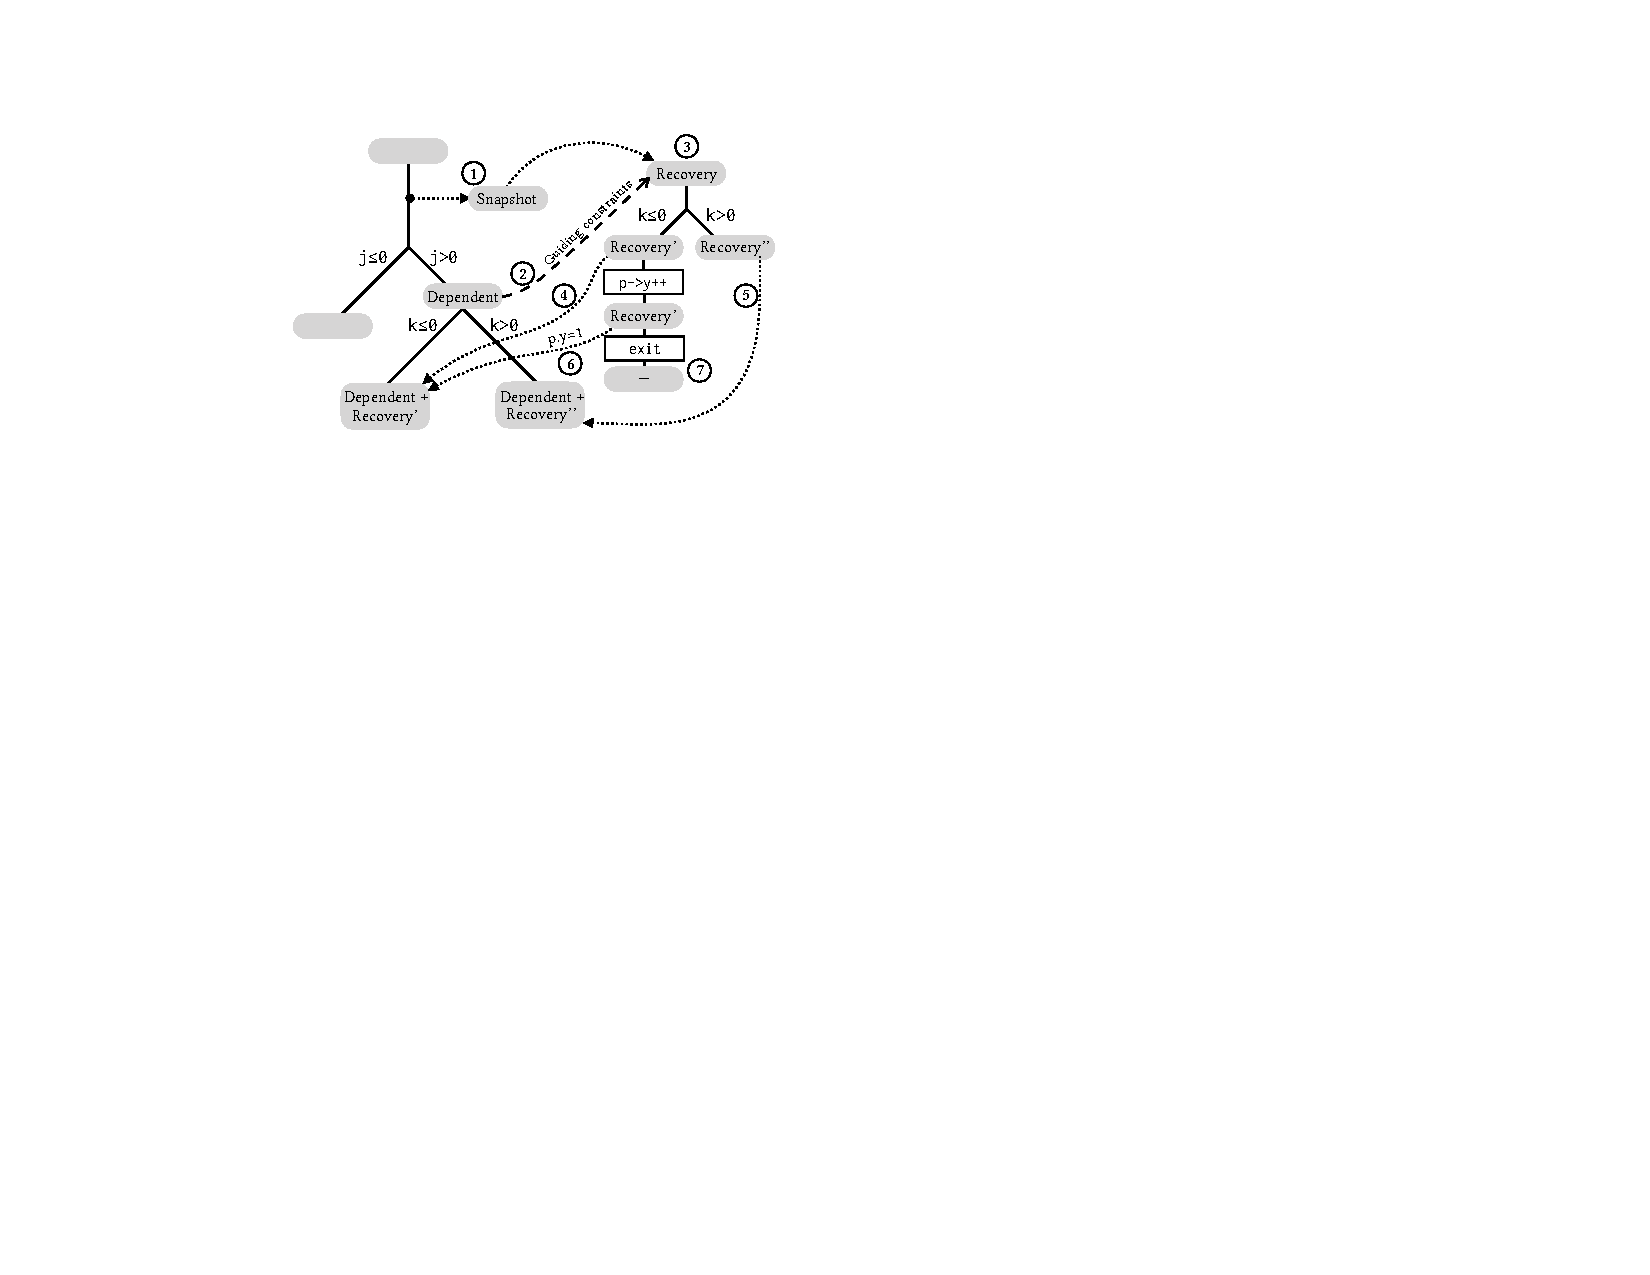
\includegraphics[width=.75\textwidth]{img-states3}}
    \label{fig:simple-fig}
  }
  \caption{Graphical illustration of chopped symbolic execution on a simple example.}
  \label{fig:simple}
\end{figure*}

%% Impact: with this form of symbolic execution we might end up
%% 1- completely skipping some code portions
%% 2- partially skipping some code portions
%% 3- not skipping the irrelevant code portions
%% In cases 2 and 3 we might still drastically reduce the
%% number of program paths and queries to the solver (due to
%% laziness in the evaluation of the skipped code)

%%% Local Variables:
%%% mode: latex
%%% TeX-master: "paper"
%%% End:

%!TEX root=./paper.tex


\chapter{Design}\label{chapter:design}

In this section, we describe our technique in detail and provide the
background regarding the main static analysis it employs, namely
\emph{pointer analysis}~\cite{andersen:pointeranalysis,
  Hind:Paste2001, Smaragdakis:FTPL2015}.

\section{TBD}

%!TEX Root=./paper.tex

\begin{algorithm} % [tbp]
\caption{Chopped symbolic execution (simplified).\label{fig:chopped-symbexe-recover}\label{fig:chopped-symbexe} }
\begin{algorithmic}[1]
  \Function{cse}{$\instate$, $\skipFunctions$}
  \State $\worklist \gets \worklist \cup \{ \instate\}$  \label{alg:seed-worklist}
  \While{$\worklist \neq \emptyset$}                     \label{alg:iterate-worklist}
    \State $\workstate \gets  \Call{selectUnsuspended}{\worklist}$ \label{alg:pop-worklist}
    \State $\inst \gets  \Call{instruction}{\workstate}$ \label{alg:get-switch-inst}

    \Switch{$\inst$} \label{alg:switch}
    \Case{Call} \label{alg:casecall-begin}
      \Call{handleCall}{$\workstate, \inst$}
    \EndCase \label{alg:casecall-end}
    \Case{Load} \label{alg:caseload-begin}
      \Call{handleLoad}{$\workstate, \inst$}
    \EndCase \label{alg:caseload-end}
    \Case{Branch} \label{alg:casebranch-begin}
      \Call{handleBranch}{$\workstate, \inst$}
    \EndCase \label{alg:casebranch-end}
    \Case{Store} \label{alg:casestore-begin}
      \Call{handleStore}{$\workstate, \inst$}
    \EndCase \label{alg:casestore-end}
    \Case{Exit} \label{alg:caseexit-begin}
      \Call{handleExit}{$\workstate, \inst$}
    \EndCase \label{alg:caseexit-end}
    \EndSwitch
  \EndWhile
  \EndFunction
\end{algorithmic}
\end{algorithm}

\begin{algorithm}
  \caption{Auxiliary procedure: \textsc{handleCall}
  \label{fig:aux-func-recS}}
\begin{algorithmic}[1]

\Function{handleCall}{$\workstate, \inst$}
\State $f \gets  \Call{targetFunction}{\workstate}$ \label{alg:call-find-target}
\If{$f \in \skipFunctions$}
  \State $\snapshot \gets \Call{createSnapshotAndSkip}{\workstate}$ \label{alg:take-snapshot}
  \State $\workstate.\skipped \gets \workstate.\skipped + (f,\snapshot,\emptyset)$ \label{alg:record-snapshot}
\Else
  \State $\Call{executeCall}{\workstate}$ \label{alg:call-normal}
\EndIf
\EndFunction
\end{algorithmic}
\end{algorithm}

\begin{algorithm}
  \caption{Auxiliary procedure: \textsc{handleLoad}
  \label{fig:aux-func-recS}}
\begin{algorithmic}[1]

\Function{handleLoad}{$\workstate, \inst$}
\State $\addr \gets \Call{loadAddress}{\workstate}$
\If{$\Call{mayMod}{\workstate,\workstate.\skipped,\addr}$}%.\skipped}$}
  %\TODO: Explain that this is a simplification and recovery states are maintained in a pool
  \State $\Call{createRecoveryState}{\workstate,\addr}$ \label{alg:call-recover}
\Else
  \State \Call{executeLoad}{$\workstate, \inst$}  \label{alg:load-normal}
\EndIf
\EndFunction
\end{algorithmic}
\end{algorithm}

\begin{algorithm}
  \caption{Auxiliary procedure: \textsc{handleBranch}
  \label{fig:aux-func-recS}}
\begin{algorithmic}[1]

\Function{handleBranch}{$\workstate, \inst$}
\If{$\workstate.\isRecovery$} \label{alg:branch-check-recovery}
  \State $\varphi = \Call{condition}{\inst}$  \label{alg:branch-get-cond}
  \State $\dependentState \gets  \Call{getDependent}{\workstate}$ \label{alg:extract-dependent}
  \State $\workstate'' \gets \Call{fork}{\workstate,\varphi }$ \label{alg:branch-fork-true1}
  \State $\dependentState'' \gets \Call{fork}{\dependentState,\varphi }$ \label{alg:branch-fork-true2}
  \If{$\Call{feasible}{\workstate''} \land \Call{feasible}{\dependentState''}$} \label{alg:branch-feasible-true}
    \State $\worklist  \gets  \worklist  \cup \{\workstate'', \dependentState''\}$ \label{alg:push-worklist-true-branch}
  \EndIf
  \State $\workstate' \gets \Call{fork}{\workstate, \neg\varphi}$ \label{alg:branch-fork-false1}
  \State $\dependentState' \gets \Call{fork}{\dependentState, \neg\varphi}$ \label{alg:branch-fork-false2}
  \If{$\Call{feasible}{\workstate'} \land \Call{feasible}{\dependentState'}$}  \label{alg:branch-feasible-false}
    \State $\worklist  \gets  \worklist  \cup \{\workstate'', \dependentState''\}$ \label{alg:push-worklist-false-branch}
  \EndIf
\Else
  \State \Call{executeBranch}{$\workstate$}  \label{alg:branch-normal}
\EndIf
\EndFunction
\end{algorithmic}
\end{algorithm}

\begin{algorithm}
  \caption{Auxiliary procedure: \textsc{handleStore}
  \label{fig:aux-func-recS}}
\begin{algorithmic}[1]

\Function{handleStore}{$\workstate, \inst$}
\State $\addr \gets \Call{storeAddress}{\workstate}$
\State $\Call{recordOverwrite}{\workstate,\addr}$     \label{alg:record-overwrite}
\State $\Call{executeStore}{\workstate,\addr}$     \label{alg:store-normal}
\If{$\workstate.\isRecovery$} \label{alg:store-check-recovery}
  \State \Call{updateDependentState}{$\workstate, \addr$} \label{alg:store-udpate-dep-states}
  \ignore{
    \If{$\addr = $\Call{dependentLoad}{$\workstate$}}
      \State $\dependentState \gets  \Call{getDependent}{\workstate}$
      \label{alg:store-extract-dependent}
      \State \Call{executeStore}{$\dependentState, \inst$}
    \EndIf
  }
\EndIf
\EndFunction
\end{algorithmic}
\end{algorithm}

\begin{algorithm}
  \caption{Auxiliary procedure: \textsc{handleExit}
  \label{fig:aux-func-recS}}
\begin{algorithmic}[1]

\Function{handleExit}{$\workstate, \inst$}
\If{$\workstate.\isRecovery \land \Call{retInSkip}{\workstate}$} \label{alg:exit-check-recovery}
  \State \Call{terminate}{$\recoveryState$} \label{alg:exit-terminate-recovery}
  \State $\dependentState \gets  \Call{getDependent}{\workstate}$ \label{alg:exit-extract-dependent}
  \State \Call{resume}{$\dependentState$} \label{alg:exit-resume}
  \State $\worklist \gets  \worklist \cup \{\dependentState\}$
\Else
  \State \Call{executeExit}{$\workstate$}  \label{alg:exit-normal}
  \label{alg:push-worklist-exit}
\EndIf
\EndFunction
\end{algorithmic}
\end{algorithm}

\begin{algorithm}
  \caption{Auxiliary procedure: \textsc{createRecoveryState}
  \label{fig:aux-func-recS}}
\begin{algorithmic}[1]

\Function{createRecoveryState}{$\workstate, \addr$}
  \ForEach{$(f,\snapshot,\owset) \in \workstate.\skipped$} \label{alg:recover-foreach}
    \If{$\Call{mayMod}{\workstate, (f,\snapshot,\owset) ,\addr}$} \label{alg:recover-if-found}
       \State $\dependentState \gets \workstate$ \label{alg:recover-gen-depS}
       \State $\Call{suspend}{\dependentState}$ \label{alg:recover-suspend}
       \State $\gc \gets  \Call{getGuidingConstraints}{\dependentState}$ \label{alg:recover-get-gc}
       \State $\recoveryState \gets \Call{fork}{\snapshot,\gc}$ \label{alg:recover-gen-recS}
       \State $\recoveryState.\isRecovery \gets \mtrue$ \label{alg:recover-set-is-recS}
       % TODO: fix the slice call...
       \State $\Call{slice}{\recoveryState,\addr}$ \label{alg:recover-slice}
       \State $\recoveryState.dependentState = \dependentState$ \label{alg:set-dependent-state}
       \State $\recoveryState.loadAddr = \addr$ \label{alg:set-load-addr}
       \State $\worklist \gets \worklist \cup \{\recoveryState\}$
       \label{alg:push-worklist-recovery}
    \EndIf
  \EndFor
\EndFunction
\end{algorithmic}
\end{algorithm}

\begin{algorithm}
  \caption{Auxiliary procedure: \textsc{mayMod}().
  \label{fig:aux-func-may-mod}}
\begin{algorithmic}[1]


\Function{mayMod}{$\workstate, \funclist, \addr$}
  \ForEach{$(f,\snapshot,\owset) \in \funclist$}
    \If{$\Call{allocSite}{\workstate,\addr} \in \Call{modSet}{f}$} \label{alg:maymod-static}
      \If{$\addr\not\in\owset$}  \label{alg:maymod-dynamic}
         \State \Return{$\mathit{true}$}
       \EndIf
    \EndIf
  \EndFor
  \State \Return{$\mathit{false}$}
\EndFunction

\end{algorithmic}
\end{algorithm}


%%% Local Variables:
%%% mode: latex
%%% TeX-master: "paper"
%%% End:


\Cref{fig:chopped-symbexe} presents the key steps in chopped
symbolic execution, which we gradually explain. The algorithm operates
on a simple imperative C-like heap-manipulating language with
assignments, assertions, conditional jumps, dynamic memory allocation
and reclamation, and function calls with call-by-value parameter
passing.\footnote{In practice, our algorithm operates on LLVM
  bitcode~\cite{llvm}.}  Functions may have pointer parameters. Thus,
without loss of generality, we assume that functions do not have a
return value.\footnote{A function with a return value can always be
  rewritten with an additional parameter that points to the memory
  location of the return value.}  To simplify the explanation, we now
assume that we may skip at most one function invocation at every
explored path, and discuss the general case in
\S\ref{Se:SkipMultipleFuncs}. For the same reason, we also assume that
the program does not dynamically allocate memory, and discuss the
handling of $\code{malloc}$ and $\code{free}$ in \S\ref{Se:Malloc}.

Chopped symbolic execution begins by invoking procedure $\textsc{cse}$
with an \emph{initial symbolic state} ($\instate$) and a set
containing the names of the functions that the user wishes to skip
($\skipFunctions$). We expect a symbolic state $\workstate$ to encode,
among other properties, the next instruction to be executed (denoted
by $\Call{instruction}{\workstate}$), the activation record stack, and
a (symbolic) description of the program \emph{heap}. For example, the
chopped symbolic execution described in \Cref{sec:overview} begins
with $\instate$ in which the stack contains only the activation record
of $\code{main}$, with the program counter at
line~\ref{line:main_enter}, an empty heap, and
$\skipFunctions = \{ \code{f} \}$.

At the beginning of the algorithm the $\worklist$ is empty, and we
initialize it with $\instate$ (\cref{alg:seed-worklist}). Then, a
standard worklist-based algorithm starts executing until either the
worklist is empty (\cref{alg:iterate-worklist}), or the algorithm
exhausts the time budget (elided). As usual, the algorithm pops the
symbolic state $\workstate$ to explore out of the worklist
(\cref{alg:pop-worklist}). Unconventionally, however, we assume that
the selected state is not suspended, as suspended states are blocked
until the value of the depended load is resolved (see
\S\ref{sec:overview}).\footnote{For simplicity, we defer the
  discussion regarding the search heuristics to \S\ref{Se:Search}, and
  assume, for now, that any unsuspended state can be returned.}  The
next step of the algorithm depends on the instruction type
(\cref{alg:switch}).

%\subsection{\caseof{Handling $\instruct{Call}$ instructions}}
\subsection{\text{Handling \textit{Call} Instructions}}
%{(lines~\ref{alg:casecall-begin}--\ref{alg:casecall-end})}}

A $\instruct{Call}$ instruction is handled as illustrated by step
\step{1} in \Cref{fig:simple} (see \S\ref{sec:overview}): First, the
algorithm determines the name $f$ of the invoked function
(\cref{alg:call-find-target}). Then, if $f$ is one of the skipped
functions, the algorithm creates a snapshot of the current state
$\workstate$ and advances the program counter in $\workstate$
(\cref{alg:take-snapshot}); records the $\snapshot$ state at the end
of its list of \emph{skipped invocations}
(\cref{alg:record-snapshot}); and returns $\workstate$ to the worklist
(\cref{alg:push-worklist-call}). A skipped invocation is represented
as a triple $(f,\snapshot,\owset)$ composed of the name of a skipped
function $f$, a $snapshot$ of the symbolic state at the time $f$ was
skipped, and a set of the addresses $\owset$ subsequently overwritten
(initially empty).

Conversely, if $f$ should not be skipped, the algorithm handles its
invocation as usual in symbolic execution.  For brevity, we elide the
standard handling of commands by symbolic execution.

\subsection{\text{Handling \textit{Load} Instructions}}
%{(lines~\ref{alg:caseload-begin}--\ref{alg:caseload-end})}

Chopped symbolic execution utilizes
$\Call{mayMod}{\workstate,\workstate.\skipped,\addr}$, shown in
\Cref{fig:aux-func-may-mod} and explained in
\S\ref{Se:IdentifyingLoads}, to determine whether the address from
which a value is read ($\addr$) might have been modified by one of the
skipped functions on the path followed by the current state
$\workstate$. If so, the algorithm generates recovery states by
calling $\Call{recover}{\workstate,\addr}$.  Otherwise, the
$\instruct{Load}$ instruction is handled as usual in symbolic
execution (\cref{alg:load-normal}).

Procedure \textsc{createRecoveryState} is shown in
\Cref{fig:aux-func-recS}. The function handles $\instruct{Load}$
instructions as illustrated by step \step{2}{} in \Cref{fig:simple}
(see \S\ref{sec:overview}): It iterates over the list of skipped
functions (\cref{alg:recover-foreach}), and uses
$\Call{mayMod}{\workstate, f,\addr}$ to determine which of the skipped
functions $f$ might have modified the dependent address. Once it finds
such a function (\cref{alg:recover-if-found}), the current state
becomes a dependent state (\cref{alg:recover-gen-depS}) and it is
immediately suspended (\cref{alg:recover-suspend}). The procedure then
generates the corresponding \emph{recovery state} $\recoveryState$ by
forking $\snapshot$ and by augmenting its path condition with the
guiding constraints $\gc$ (\cref{alg:recover-get-gc}), \ie the path
conditions accumulated in $\workstate$ since the snapshot state was
created (\cref{alg:recover-gen-recS,alg:recover-set-is-recS}). The
algorithm then invokes a static program slicer to remove from the
skipped function $f$ instructions which cannot affect the address of
the dependent load (\cref{alg:recover-slice}); records that
$\recoveryState$ was spawned to determine the value written in address
$\addr$ of $\dependentState$ (\cref{alg:recover-record-dep}); and
pushes the two states into the worklist
(\cref{alg:push-worklist-recovery}).

\subsection{\text{Handling \textit{Branch} Instructions}}
%{(lines~\ref{alg:casebranch-begin}--\ref{alg:casebranch-end})}

The algorithm checks whether the current state $\workstate$ is a
recovery state. If so, then the $\instruct{Branch}$ instruction is
handled as illustrated by steps \step{4}{} and \step{5}{} in
\Cref{fig:simple} (see \S\ref{sec:overview}): It first extracts from
the worklist the (suspended) dependent state $\dependentState$, which
spawned $\workstate$ as a recovery state
(\cref{alg:extract-dependent}).  It then determines the branch
condition $\varphi$ (\cref{alg:branch-get-cond}); forks both the
current (recovery) state $\workstate$ and the dependent state
$\dependentState$, and adds $\varphi$ to their path condition
(lines~\ref{alg:branch-fork-true1}--\ref{alg:branch-fork-true2}).
After the fork, it checks whether the resulting states are feasible,
\ie their path conditions are satisfiable
(\cref{alg:branch-feasible-true}), and if so, adds them to the
worklist. If either one is not feasible, the newly forked recovery and
dependent states are simultaneously discarded
(\cref{alg:push-worklist-true-branch}).
Lines~\ref{alg:branch-fork-true1}--\ref{alg:push-worklist-true-branch}
act similarly to
lines~\ref{alg:branch-fork-false1}--\ref{alg:push-worklist-false-branch},
except that we use the negation of the branch condition
$\neg\varphi$. If the current state $\workstate$ is not a recovery
state, then the $\instruct{Branch}$ instruction is handled as usual in
symbolic execution (\cref{alg:branch-normal}).

\subsection{\text{Handling \textit{Store} Instructions}}
%{(lines~\ref{alg:casestore-begin}--\ref{alg:casestore-end})}

The algorithm executes the $\instruct{Store}$ instruction on the
current state in two steps. First, it updates the set of overwritten
addresses of the skipped function to record that a value was stored in
$\addr$ after the skip, and thus any value they may write is no longer
relevant (\cref{alg:record-overwrite}). Lastly, the symbolic state
$\workstate$ is updated as usual in symbolic execution
(\cref{alg:store-normal}). If $\workstate$ is a recovery state, then
the algorithm invokes
\Call{udpateDependentStates}{$\workstate, \addr$} (code elided) to
updated the dependent state (as illustrated by step \step{6}{} in
\Cref{fig:simple}, see \S\ref{sec:overview}). In addition, it also
updates the set of overwritten addresses in the list of skipped
invocations of the dependent state. Note that
\Call{udpateDependentStates}{$\dependentState, \inst$} updates, but
does not resume, the dependent state.

\subsection{\text{Handling \textit{Exit} Instructions}}
%{(lines~\ref{alg:caseexit-begin}--\ref{alg:caseexit-end})}

The algorithm checks whether the current state $\workstate$ is a
recovery state. If $\workstate$ is a recovery state \emph{and} the
$\instruct{Exit}$ instruction is invoked inside the skipped function,
then the recovery is terminated and the instruction is handled as
illustrated by step \step{7}{} in \Cref{fig:simple} (see
\S\ref{sec:overview}): Specifically, the recovery state itself if
discarded (\cref{alg:exit-terminate-recovery}) and the dependent state
is resumed \cref{alg:exit-resume}. Otherwise, the $\instruct{Exit}$
instruction is handled as usual in symbolic execution
(\cref{alg:exit-normal}).


%!TEX root=./paper.tex

\subsection{Static Inference of Function Side-Effects}
\label{Se:MayMod}
\label{Se:IdentifyingLoads}

The auxiliary function $\Call{mayMod}{ \workstate, \funclist, \addr }$
receives as parameters a symbolic state $\workstate$, a list of
skipped invocations $\funclist$, and an address $\addr$ which is the
target of a $\instruct{Load}$ instruction, and determines whether one
of the skipped function in $\funclist$ may store a value in $\addr$.
The function makes this decision using a \emph{points-to} graph
computed by a preliminary stage of pointer
analysis~\cite{Hind:Paste2001, Smaragdakis:FTPL2015}.

More specifically, we perform a whole program flow-insensitive,
context-insensitive, and field-sensitive points-to analysis which
determines, in a conservative way, the memory location each pointer
variable may point-to. In this analysis, memory locations are
conservatively abstracted using their \emph{allocation sites}: Every
definition of a local or a global variable is considered to be an
allocation site, as well as every program point in which memory is
allocated. For example, if the program contains
$\code{while (..) do L: p=malloc(4)}$ then we represent all the memory
locations allocated in $L$ by a single allocation site
$\mathit{AS}_L$.  We then say that $\code{p}$ may point to allocation
site $\mathit{AS}_L$, and if the program contains $\code{p=q}$, we say
the same about $\code{q}$. The nodes of the points-to graph of a
program are the variable names and allocation sites, and its edges
represent \emph{points-to relations}: An edge from node $v$ to $w$
means that the memory location represented by $v$ may hold a pointer
to $w$.

The points-to graph, which is computed once for every program,
conservatively represents all the possible points-to relation in any
possible program execution. Using the points-to graph, we use a
standard \emph{may-mod} analysis (see, e.g.,~\cite{dragon-book}), in
which we find the side effects of every function $f$, \ie the set of
possible locations, represented by their allocation sites, that the
function itself or any function that it may (transitively) invoke, may
modify.

During the chopped symbolic execution, we instrument the symbolic
state to record the allocation site of every memory location. This
instrumentation, together with the program points-to graph, allows
\textsc{mayMod} to determine whether a skipped function may write to a
given address. Recall that the pointer analysis is flow-insensitive,
and thus it might record that a skipped function might modify a
location which is updated later on in the symbolic execution.  More
specifically, a $\instruct{load}$ instruction from address $\addr$ is
\emph{dependent on an invocation of a skipped function} if and only
if: (1)~$\addr$ is among the locations that \textit{may} be modified
by the skipped function (according to the may-mod analysis), and
(2)~no stores to that location happened between the skipped invocation
function and the load. In particular, when the second condition
doesn't hold, no recovery is needed as the stores performed by the
skipped function are irrelevant. $\Call{mayMod}$ utilizes the
information gathered during the symbolic execution regarding
overwritten locations to refine on-the-fly the detection of the
\emph{relevant} side effects of skipped functions.

\subsection{Multiple Recovery States}
\label{Se:MultiRecovery}
In some cases, we need to create several recovery states during a
single chopped symbolic execution.

For example, consider the following code fragment which modifies the
body of the \code{main()} function in Figure~\ref{fig:simple}:
\[
\code{f(\&p,k); if (p.x) \{ p.z++; \} if (p.y) \{ p.z--; \}}
\]
If we wish to skip the invocation to $\code{f}()$ then a recovery
state and a dependent state are created every time the condition of
the branch needs to be evaluated. Note that the second dependent state
is produced from the first dependent one and that the resumed state
encapsulates the changes made by the first recovery state. Assume that
these changes involve a modification of the value of $\code{p.x}$
inside the $k>0$ branch at line~\ref{line:px_write}. If the symbolic
execution of the second recovery state goes through the path in which
$\code{p.y}$ is updated ($k\le0$), the induced combined execution
would be infeasible. To avoid this undesirable situation, when a
recovery state terminates, it adds the new constraints accumulated in
its path condition to the \textit{guiding constraints} of its dependent state. The added
constraints are then used in subsequent recovery states. In our
example in Figure~\ref{fig:simple}, the constraint $k > 0$ is
propagated from the first recovery state to the first dependent state,
thus ensuring that the symbolic execution of the second recovery state
does not follow an infeasible path.

%!TEX root=./paper.tex

\subsection{Handling Multiple Skipped Functions}
\label{Se:SkipMultipleFuncs}
So far, we have assumed that every symbolic state has a single skipped
invocation. When we have multiple invocations that can be skipped, we
then need to decide which functions to use for recovery and in which
order, in the case multiple invocations modify the dependent load
address $\addr$. We solve this issue by executing the skipped
invocations according to their order along the path, thus ensuring
that the value stored in $\addr$ at the end of the recovery process is
indeed the last value written there along the chopped path.

Another issue that we need to address to support multiple skipped
functions is that a skipped invocation might depend on the side
effects of an earlier skipped functions. When this happens, we apply
our recovery approach in a recursive manner, and treat the current
recovery state as a \emph{dependent} state. For example, consider the
code in Figure~\ref{fig:multiple-skipped-functions}. When the
execution reaches the dependent load at line~13, we create a recovery
state for $\code{f}_2$, since $\code{f}_1$ does not modify the field
$x$.  When the created recovery state reaches the load instruction at
line~6, it identifies it as a dependent load. Chopped symbolic
execution then creates another recovery state which executes $f_1$.
Once the recovery of $f_1$ is terminated, we can continue with the
recovery of $f_2$.

To make the symbolic execution more efficient in these cases, we
maintain for each state a cache which records the recovery states
which were actually relevant for any given load. By doing this, we can
avoid redundant recovery executions.

\begin{figure}[tbp]
\lstinputlisting[linewidth=.95\columnwidth]{code/multiple-skipped.c}
\caption{Multiple skipped functions.}\vspace{-5mm}
\label{fig:multiple-skipped-functions}
\end{figure}

%%% Local Variables:
%%% mode: latex
%%% TeX-master: "paper"
%%% End:


%!TEX root=./thesis.tex

\section{Memory allocations}
\label{Se:Malloc}

Let us consider the example from
Figure~\ref{fig:slices-with-allocations}, where the skipped function
\code{f} allocates memory with \code{malloc}. After skipping the
function call at line~\ref{line:alloc_skip}, the chopped symbolic
execution encounters two dependent loads at
lines~\ref{line:alloc_first} and \ref{line:alloc_second}. Chopped
symbolic execution thus spawns two consecutive recovery states: one in
which executes only line~\ref{line:slice_1}, and one in which executes lines~\ref{line:slice_1} and
lines~\ref{line:slice_2}. If we allowed \code{malloc} to return two different addresses while
executing the recovery states, this may lead to undefined behavior
since the second recovery would write to a different memory
address. To prevent this, and maintain consistency across recovery
states originating from the same function call, we maintain a list of
returned addresses for each allocation site in \code{f} which are
identified by their call stack. This way, subsequent recovery states
will use this information while re-executing allocating instructions.

\begin{figure}[tbp]
  \lstinputlisting[linewidth=.95\columnwidth]{code/allocations.c}\vspace{-2mm}
  \caption{Example of skipped function with allocation.}\vspace{-4mm}
\label{fig:slices-with-allocations}
\end{figure}

%%% Local Variables:
%%% mode: latex
%%% TeX-master: "paper"
%%% End:


%!TEX root=./paper.tex

\subsection{Chopping-Aware Search Heuristics}
\label{Se:Search}

Search heuristics are the main approach to reduce path explosion and
steer symbolic execution to uncovered paths for a more effective
exploration~\cite{exe,klee,sen:concolicheuristics,fitsymex:dsn09}, and
chopped symbolic execution is no exception. However, these heuristics
do not take into account the particular nature of the states in
chopped symbolic execution, that is the distinction between normal and
recovery states.

We propose a \textit{chopping-aware} search heuristic, which attempts
to optimize the exploration of chopped symbolic execution, while
aiming to a faster recovery of side effects. The heuristic's behavior
crucially depends on the current state being executed. Under normal
conditions---that is while symbolically executing normal states---the
search heuristic favors the selection of normal states at the next
steps. The rationale is that we want to favor paths that do not
require any recovery, thus fostering code exploration.

Instead, when chopped symbolic execution is executing a recovery
state, the search heuristic only selects the recovery states involved
in the recovery process. In this case, we want to favor a fast
recovery of the side effects needed by the dependent state. As soon as
the recovery state terminates, the search heuristic will switch to the
normal behavior.

Since always favoring normal states over recovery states may lead to
saturation in code exploration, we allow the searcher to select at a
lower probability a recovery state even under normal execution
conditions.

%%% Local Variables:
%%% mode: latex
%%% TeX-master: "paper"
%%% End:


%%% Local Variables:
%%% mode: latex
%%% TeX-master: "paper"
%%% End:


%%% Local Variables:
%%% mode: latex
%%% TeX-master: "paper"
%%% End:

%!TEX root=./thesis.tex

\chapter{Implementation}\label{chapter:implementation}

We implemented chopped symbolic execution into \toolname, an extension
to the KLEE symbolic execution
engine~\cite{klee}.\footnote{http://url-omitted-for-double-blind-revision}
Our KLEE extension starts from commit~\code{b2f93ff}.
Our implementation, which includes various static analyses
and an extension to the symbolic execution engine,
consists of 4500 lines of C++ code.
A user can run \toolname by
specifying the list of functions to skip along with specific call
sites via command-line switches.

\section{Static Analysis}
Our tool combines static analysis, in particular mod-ref analysis and slicing
along with symbolic execution.
Since KLEE operates on LLVM bitcode, we rely on libraries
that statically analyze LLVM bitcode.
In particular, we implemented a code base for static analyses that exposes APIs to KLEE, so new or
better static analyses can be integrated in \toolname with ease.

\subsection{Mod-Ref Analysis}
We compute \textit{mod-ref analysis} by using the pointer analysis
provided by SVF~\cite{sui2016svf}. In particular, we rely on a
flow-insensitive and context-insensitive pointer analysis based on the
Andersen algorithm~\cite{andersen:pointeranalysis}.
Based on the pointer analysis results,
we compute an approximation of the control flow graph
which is used while computing the side effects of a given function.
The \textit{modifies}-set of a function $f$ is computed
by collecting the points-to information of all the $store$ instructions of the functions which
are reachable from $f$, according the our approximated control flow graph.
As for the \textit{ref}-set of $f$, we first identify all the call sites of $f$
and then collect the points-to information from all the $load$ instructions which are reachable
from these call sites (again, based on the approximated control flow graph).
The side effects of $f$ are given by the intersection of the \textit{modifies}-set and the \textit{ref}-set.

\subsection{Static Slicing}
We compute static backward slicing using the DG static slicer~\cite{dg}.
A static slicing criterion is given by a line and a set of variables.
In DG, the slicing criterion is expressed by placing a call site with parameters.
The call site corresponds to the line and the parameters correspond to the variables.
A \textit{load} instruction which dependends on the side effects of a skipped function
is associated with the \textit{store} instructions which may modify the relevant memory location.
Each such \textit{store} instruction is annotated with a call to a unique function,
which is passed as a criterion for the static slicer.
We modified the slicer to be able to generate slices of arbitrary functions and not
only of the entry point of the program. Note that static slicing is
computed on-demand, only when a recovery is required. The same slice
may be reused for multiple recoveries, so each slice is computed only
once.

\subsection{Inlining}
Since our pointer analysis is context-insensitive,
inlining common functions (mostly, library functions) can result in better precision.
The inlining is prefromed only in the functions which are reachable from any skipped function.
This partial inlining prevents to code from growing too much.
A user can specifiy the functions for inlining via a command line option.

\subsection{Handling Non Void Functions}
If all the skipped funtions would have no return value,
then we were able to run the mod-ref analysis by inspecting only \textit{load} and \textit{store} instructions.
Unfortunately, that is not the situation in practice.
In order to handle this, we perform a reduction from a returning function to a non-returning function.
Suppose that we have the following returning function:
\begin{lstlisting}[linewidth=.4\textwidth,numbers=none]
int f(int x, int y) {
    return x + y;
}
\end{lstlisting}
\label{fig:ret2void-original}
We create a non-returning wrapper function $wf$ as follows:
\begin{lstlisting}[linewidth=.4\textwidth,numbers=none]
void wf(int *result, int x, int y) {
    *result = f(x, y);
}
\end{lstlisting}
\label{fig:ret2void-original}
Once we have the wrapper function, we replace the calls for $f$ with calls for $wf$.
If the original usage of $f$ was:
\begin{lstlisting}[linewidth=.4\textwidth,numbers=none]
int z = f(x, y);
\end{lstlisting}
then it is rewritten to:
\begin{lstlisting}[linewidth=.4\textwidth,numbers=none]
int result;
wf(&result, x, y);
int z = result;
\end{lstlisting}
We implemented an LLVM pass which does these rewritings automatically.

\section{Symbolic Execution}
In order to have \textit{recovery} and \textit{normal} states,
we extended the symbolic execution state
and added additional properties: \textit{guiding constraints, owset, allocation record}, \etc (see~\Cref{chapter:design}).
When the slicing of a function $f$ is required,
we create an inclusive clone of $f$ (considering the reachable functions from $f$).
The slicing is performed on the cloned functions, which are later added dynamically to KLEE's functions.
We modified the handling of the \textit{call} instruction,
such that we would be able to inject calls to the sliced functions as well as to the original ones.


\subsection{State Exploration}
\toolname also implements its own state
prioritization algorithm, \textit{chopped-aware search heuristic},
which favors the execution of normal states over recovery ones as
discussed in \S~\ref{Se:Search}. The algorithm is implemented as a
\textit{state searcher}, an abstraction used by KLEE to encapsulate
the state exploration logic. This implementation strategy also allows
us to be search-heuristic agnostic, meaning that our prioritization
strategy is compatible and can be combined with all present and future
search heuristics of KLEE.

\section{Limitations}
The current main limitation of \toolname is
the handling of symbolic addresses. Handling a symbolic address in
\toolname is not trivial, as it may refer to multiple allocation sites
and in turn lead to the recovery of several different skipped
functions. Moreover, symbolic addresses also increase the complexity
of interpreting load instructions. In case of a load instruction,
\toolname needs a concrete address to update in the dependent state
the addresses written during recovery, as discussed in \Cref{chapter:design}.

Chopped symbolic execution currently focuses on skipping functions.
However, the approach is more generic: In theory, we could skip any
arbitrary code portion that preserves the control-flow of the
program. We are currently working on relaxing the implementation of
\toolname to support such feature, and on designing an appropriate API
for specifying such arbitrary code portions.

%%% Local Variables:
%%% mode: latex
%%% TeX-master: "thesis"
%%% End:

%!TEX root=./paper.tex

\chapter{Experiments}\label{chapter:experiments}

Our evaluation aims to provide preliminary evidence that this novel
form of symbolic execution can lead to significant scalability
gains. In particular, we evaluate its effectiveness when embodied in
the following two scenarios:

\begin{enumerate}[leftmargin=*]
\item \textbf{Failure reproduction}, where the research question we
  explore is: How does chopped symbolic execution perform with respect
  to standard symbolic execution in generating an input that triggers
  a failure? In particular, can it reproduce more failures than standard
  symbolic execution, or can it reproduce the same failures faster?

\item \textbf{Test suite augmentation}, where the research question we
  explore is: How does chopped symbolic execution perform when steered
  to generate test cases that improve the structural coverage of code?
  Can chopped symbolic execution complement the exploration of
  standard symbolic execution?
\end{enumerate}

Note that our objective is not to claim that chopped symbolic
execution is generally a superior technique for a specific task---and
thus omits a direct comparison with other state-of-the-art techniques
for each scenario---but rather to assess the attainable benefits of
chopped symbolic execution when applied to techniques built upon
symbolic execution engines.

We compare \toolname with baseline KLEE. We use the same KLEE commit
(\texttt{b2f93ff}) from which we based \toolname.  Both tools are
compiled with LLVM 3.4.2~\cite{llvm} and use STP 2.1.2 as the
constraint solver~\cite{stp}. We conduct our experiments on two
identical servers running Ubuntu 14.04, equipped with an 8-core Intel
processor at 3.5 GHz and 16GB of RAM.

\section{Failure Reproduction}\label{sec:disc-secur-vuln}
In this experiment we use chopped symbolic execution for failure
reproduction. In particular, we run a symbolic executor to generate
inputs that trigger known security vulnerabilities.

\begin{table}[tbp]
  \caption{Security vulnerabilities in \textsf{libtasn1} considered
    for reproduction, with version used and number of lines of code.}
\begin{tabular}{|l|c|r|}
  \hline
  \textbf{Vulnerability} & \textbf{Version} & \textbf{C SLOC} \\ \hline
  CVE-2012-1569 & 2.11& 24,448 \\ \hline
  CVE-2014-3467 & 3.5 & 22,091 \\ \hline
  CVE-2015-2806 & 4.3 & 28,115 \\ \hline
  CVE-2015-3622 & 4.4 & 28,109 \\ \hline
\end{tabular}
\label{tab:vuln-stats}
\end{table}

\subsection{Benchmarks}
The subjects of this part of the evaluation are
vulnerabilities taken from GNU \textsf{libtasn1}. As briefly discussed
in the introduction, GNU \textsf{libtasn1} is a library for
serializing and deserializing data in Abstract Syntax Notation One
(ASN.1) format.  For example, \textsf{libtasn1} is used in GnuTLS to
define X.509 certificates.  We selected the \textsf{libtasn1} library
because its code is complex, with nested and deep function calls, and
can be successfully analyzed by the KLEE symbolic executor.
Table~\ref{tab:vuln-stats} lists and briefly characterizes the
vulnerabilities selected for our experiment, which are memory
out-of-bounds accesses.  Note that each vulnerability requires the
reproduction of a single failure, except for CVE-2014-3467, for which
the vulnerability can be exploited in three different code locations,
so we consider three different failures.  Therefore, in this
experiment we aim to reproduce a total of 6 failures.

\subsection{Methodology}
We proceed with the following evaluation process:

\begin{enumerate}[leftmargin=*]
\item We manually create an execution driver for the \textsf{libtasn1}
  library to exercise the library from its public interface,
  simulating the interactions of an external program (\eg GnuTLS).
\item We manually derive the set of functions to skip by inspecting
  the code, and the vulnerability report that usually includes the
  stack trace and sometimes results from a dynamic analysis tool (\eg
  Valgrind~\cite{valgrind2003}). For the selected case studies we
  managed to identify a candidate set of function to exclude in less
  than 30 minutes per failure, but a developer familiar with the code
  should be able to do so faster.
\item We invoke KLEE and \toolname on the subject with several
  different search heuristics (random, DFS, and coverage-based) and a
  time limit of 24 hours. We also configure the symbolic executors to
  terminate the execution as soon as the vulnerability is
  identified. We do that by adding a new option to KLEE that, given a
  list of code locations, terminates the execution as soon as a
  vulnerability is discovered at all locations.
\end{enumerate}

Note that we initialize the pseudo-random number generator of the
random heuristic with the same seed, thus obtaining the same
exploration between consecutive runs and allowing for a fair
comparison between KLEE and \toolname.

\subsection{Results}
Table~\ref{tab:vulnerability-table} summarizes the high-level results
of our failure reproduction experiment. For each vulnerability and
search heuristic we report the effectiveness of KLEE and \toolname at
reproducing the failure as the time required to generate an input that
triggers the vulnerability.
% For \toolname we report for each
% vulnerability the best result among all validated configurations (more
% details later).

As can be seen, \toolname outperforms KLEE on all but one case study
both in terms of number of failures reproduced and performance,
regardless of the search heuristic applied. Overall, KLEE reproduces
four failures, CVE-2014-3467$^1$, CVE-2014-3467$^2$, CVE-2015-2806 and
CVE-2015-3622, and only failure CVE-2014-3467$^1$ can be reproduced
with all search heuristics. This latter case seems to be relatively
easy to identify, since KLEE requires only a few seconds. On the other
cases, KLEE requires between 1 and 20 hours. The problem of path
explosion in KLEE is particularly visible in CVE-2012-1569 where the
symbolic executor quickly runs out of available memory (4096 MB) and
thus fails to reproduce the failure.

In contrast, \toolname can identify all vulnerabilities and generates
a test case to reproduce each failure in less than 20 minutes, and
often much faster. Overall, for the vulnerabilities that KLEE can also
reproduce, CHASER can significantly beat KLEE in terms of performance
by at least an order of magnitude, with the only exception of
CVE-2014-3467$^1$ where \toolname can be slowed by the cost of static
analyses.

Table~\ref{tab:vulnerability-table-chaser} summarizes the detailed
results of \toolname for the failure reproduction experiment. For each
vulnerability and search heuristic we report the number of snapshots
and recovery states generated during chopped symbolic execution
(Snapshots and Recoveries, respectively), the execution times for
\toolname with and without slicing (Sliced $\mathcal{F}$ and Full
$\mathcal{F},$ respectively) as well as statistics on the generated
slices, which includes the number of slices generated (Num), and the
total size of the original ($\mathcal{F}$ size) and sliced
($\mathcal{S}$ size) skipped functions in terms of LLVM instructions.

Table~\ref{tab:vulnerability-table-chaser} shows that the number of
skipped functions (as deduced by the number of snapshot states) and
recovery states varies with the nature of the case study, the skipped
functions, and the search heuristic. In the case of vulnerability
CVE-2015-2806, \toolname could reproduce the failure without
recovering. This is the exemplar case that highlights the benefits of
chopped symbolic execution: While KLEE spent hours interpreting code
unrelated with the failure, \toolname excluded the uninteresting code
portions and could proceed analyzing only code of interest,
consistently identifying the failure with all search heuristics in as
little as one minute.

Table~\ref{tab:vulnerability-table-chaser} also shows that the benefit
of slicing the skipped functions depends on the case study. For
example, for the CVE-2014-3467$^3$ vulnerability, \toolname is on
average 70\% faster when slicing the skipped functions. Conversely,
\toolname performs the best without slicing in CVE-2012-1569. A
plausible explanation is that the additional analyses required for
slicing were more expensive than directly analyzing the functions. We
plan to develop a lightweight analysis to speculatively identify when
to apply slicing on the skipped functions.

\begin{table}[t]
  \caption{Results for the failure reproduction experiment for KLEE
    and \toolname on libtasn1. For each case we report the number of
    successful failures reproduced and the time required for the
    exploration (in \textit{hh:mm:ss}).}
\begin{tabular}{|l|C{1.4cm}|R{1.4cm}|R{1.4cm}|}
  \hline
  \textbf{Vulnerability} & \textbf{Search} & \makecell[c]{\textbf{KLEE}} & \makecell[c]{\textbf{\toolname}} \\ \hline\hline

  \multirow{3}{*}{CVE-2012-1569}
   & Random   & $\dagger$~11:52 & 02:27 \\ \cline{2-4}
   & DFS      & $\dagger$~05:08 & 03:29 \\ \cline{2-4}
   & Coverage & $\dagger$~11:28 & 02:45 \\
  \hline\hline

  \multirow{3}{*}{CVE-2014-3467$^1$}
   & Random   & 00:05 & 00:45 \\ \cline{2-4}
   & DFS      & 16:31 & 00:08 \\ \cline{2-4}
   & Coverage & 00:03 & 00:58 \\
  \hline\hline

  \multirow{3}{*}{CVE-2014-3467$^2$}
   & Random   &          1:02:13 & 06:18 \\ \cline{2-4}
   & DFS      & \textit{Timeout} & 00:09 \\ \cline{2-4}
   & Coverage &          1:33:56 & 02:48 \\
  \hline\hline

    \multirow{3}{*}{CVE-2014-3467$^3$}
   & Random   & \textit{Timeout} & 09:55 \\ \cline{2-4}
   & DFS      & \textit{Timeout} & 12:31 \\ \cline{2-4}
   & Coverage & \textit{Timeout} & 09:50 \\
  \hline\hline

  \multirow{3}{*}{CVE-2015-2806}
   & Random   &      1:07:46 & 02:18 \\ \cline{2-4}
   & DFS      &      2:46:13 & 12:04 \\ \cline{2-4}
   & Coverage &$\dagger$~38:56 & 01:02 \\
  \hline\hline

  \multirow{3}{*}{CVE-2015-3622}
   & Random   &  \textit{Timeout} & 00:16 \\ \cline{2-4}
   & DFS      &  \textit{Timeout} & 18:41 \\ \cline{2-4}
   & Coverage & 20:25:20 & 00:18 \\
  \hline
\end{tabular}
\flushleft
\begin{tabular}{L{\columnwidth}}
  \textit{Timeout}: Execution terminated after 24 hours \\
  $\dagger$ Execution terminated due to memory exhaustion \\
\end{tabular}\vspace{-5mm}
\label{tab:vulnerability-table}
\end{table}

\begin{table*}[t]
  \caption{Detailed results of \toolname for the failure reproduction
    experiment on libtasn1.}
{\def\arraystretch{0.9}
\begin{tabular}{|L{2.2cm}|C{1.5cm}|R{1.5cm}|R{1.6cm}|rr|rrr|}
  \hline
  \multirow{2}{*}{\textbf{Vulnerability}} & \multirow{2}{*}{\textbf{Search}} & \multirow{2}{*}{\makecell[c]{\textbf{Snapshots}}} & \multirow{2}{*}{\makecell[c]{\textbf{Recoveries}}} & \multicolumn{2}{c|}{\textbf{Function}} & \multicolumn{3}{c|}{\textbf{Slice}} \\
  & & & & \makecell[c]{\textbf{Full $\mathcal{F}$}} & \makecell[c]{\textbf{Sliced $\mathcal{F}$}} & \textbf{Num} & \makecell[c]{\textbf{$\mathcal{F}$ Size}} & \makecell[c]{\textbf{$\mathcal{S}$ Size}}\\ \hline\hline

  \multirow{3}{*}{CVE-2012-1569}
   & Random   & 5,315 & 7,447    & 01:21 & 02:27 & 4 & 694 & 320 (46\%)\\ \cline{2-9}
   & DFS      &   381 & 1,078    & 00:10 & 03:29 & 4 & 694 & 320 (46\%)\\ \cline{2-9}
   & Coverage & 6,258 & 9,053    & 01:53 & 02:45 & 4 & 694 & 320 (46\%)\\ \cline{2-9}
  \hline\hline

  \multirow{3}{*}{CVE-2014-3467$^1$}
   & Random   &  6,607 & 6,883   &00:30 &00:45 & 4 & 3,740 & 2,318 (62\%) \\ \cline{2-9}
   & DFS      &    656 & 1,003   &00:07 &00:08 & 4 & 3,740 & 2,318 (62\%) \\ \cline{2-9}
   & Coverage &  5,642 & 7,357   &00:50 &00:58 & 4 & 3,740 & 2,318 (62\%) \\ \cline{2-9}
  \hline\hline

  \multirow{3}{*}{CVE-2014-3467$^2$}
   & Random   & 16,279 & 26,300   &07:38 &06:18 & 4 & 3,740 & 2,318 (62\%) \\ \cline{2-9}
   & DFS      &    656 &  1,003   &00:11 &00:09 & 4 & 3,740 & 2,318 (62\%) \\ \cline{2-9}
   & Coverage & 10,147 & 18,916   &04:43 &02:48 & 4 & 3,740 & 2,318 (62\%) \\ \cline{2-9}
  \hline\hline

    \multirow{3}{*}{CVE-2014-3467$^3$}
   & Random   & 26,762 & 43,480   &17:30 &09:55 & 4 & 3,740 & 2,318 (62\%) \\ \cline{2-9}
   & DFS      & 38,696 & 61,113   &17:07 &12:31 & 4 & 3,740 & 2,318 (62\%) \\ \cline{2-9}
   & Coverage & 30,947 & 42,797   &17:13 &09:50 & 4 & 3,740 & 2,318 (62\%) \\ \cline{2-9}
  \hline\hline

  \multirow{3}{*}{CVE-2015-2806}
   & Random   &   173,065 & 0   & 02:31 & 02:18 & - & - & -\\ \cline{2-9}
   & DFS      & 2,708,849 & 0   & 12:30 & 12:04 & - & - & -\\ \cline{2-9}
   & Coverage &    36,549 & 0   & 01:04 & 01:02 & - & - & -\\ \cline{2-9}
  \hline\hline

  \multirow{3}{*}{CVE-2015-3622}
   & Random   &    584 &  8,980   & 00:25 & 00:16 & 6 & 1,269 & 343 (27\%)\\ \cline{2-9}
   & DFS      & 23,846 & 20,188   & 21:24 & 18:41 & 7 & 1,453 & 398 (27\%)\\ \cline{2-9}
   & Coverage &    608 &  9,043   & 00:23 & 00:18 & 6 & 1,269 & 343 (27\%)\\ \cline{2-9}
  \hline
\end{tabular}}
\label{tab:vulnerability-table-chaser}
\end{table*}

%%% Local Variables:
%%% mode: latex
%%% TeX-master: "../paper"
%%% End:


\section{Test Suite Augmentation}
\label{sec:code-cover-impr}
In this experiment we use chopped symbolic execution for test suite
augmentation. We do that by running \toolname on a subject program
where we skip functions already exercised by an existing test
suite. As initial test suite we rely on tests generated by KLEE. In
essence, we want to assess the effectiveness of chopped symbolic
execution in complementing standard symbolic execution in test
generation, ultimately increasing structural coverage.

\subsection{Benchmarks}
The subjects of this part of the evaluation are
GNU \textsf{BC} 2.27 and \textsf{LibYAML}. \textsf{BC} is an
arbitrary-precision calculator that solves mathematical expressions
written in a C-style language.  \textsf{LibYAML} is a well-known
library for parsing and emitting data in YAML format, which is a human
friendly data serialization standard.  We choose \textsf{BC} and
\textsf{LibYAML} because KLEE has a hard time generating high-coverage
tests. As a result, the code not covered by KLEE is usually related to
complex features, and we challenge \toolname to exercise it. For each
program, we rely on the program's documentation and personal
experience with the subject to identify the best argument
configuration that can maximize coverage.

\subsection{Methodology}
We proceed with the following evaluation process:

\begin{enumerate}[leftmargin=*]
\item We generate the initial test suite by running KLEE on each
  subject with coverage-based search heuristic and a time limit of one
  hour. We use this configuration to maximize structural coverage of
  the code under analysis, in particular we focus on statement and
  branch coverage.
\item We compute the structural coverage obtained with the test suites
  that KLEE generates using GNU
  GCov.\footnote{https://gcc.gnu.org/onlinedocs/gcc-4.7.3/gcc/Gcov.html}
\item We use the coverage information and the call graph to select for
  each program the set of functions to skip based on the coverage
  information. For example, suppose that function $f$ calls function
  $g$ and $h$, and that $f$ and $h$ are covered by a test. We include
  in the set of the skipped functions only $h$, since $f$ is required
  to reach uncovered function $g$.
\item We invoke \toolname on the subjects with coverage-based search
  heuristic and a time limit of one hour.
\end{enumerate}

\subsection{Results}
Table~\ref{tab:experiments-table-augmentation} summarizes the results
of our test suite augmentation experiment. For each case study we
report the structural coverage of a symbolic executor as percentage of
statements (Lines) or branches (Branches) covered by its generated
test suite. For CHASER we report the structural coverage results with
and without performing slicing (Sliced $\mathcal{F}$ and Full
$\mathcal{F}$, respectively).

Table~\ref{tab:experiments-table-augmentation} shows that \toolname
effectively complements KLEE and increases code coverage even on
complex subjects. Specifically, on \textsf{BC}, \toolname increased
statement and branch coverage by +2.43\% and +3.16\%, respectively,
and on \textsf{LibYAML} it more than doubled statement coverage (from
10.8\% to 22.6\%) and more than tripled branch coverage (from 4.2\% to
15\%).

In \textsf{LibYAML} we observed that KLEE spent almost all its budget
analyzing one function that contains complex logic responsible for
ensuring that the buffer contains enough characters for parsing while
handling different encodings, such as UTF-8 or UTF-16. Such function
is invoked at the beginning of program execution, and KLEE got stuck
into it, not being able to execute any subsequent line of
code. Conversely, \toolname skipped the expensive invocation and
continued to explore other parts of the code. Our chopping-aware
search heuristic also allowed us to recover paths inside the expensive
function while giving higher priority to non-recovery states, in turn
resulting in a more in-depth exploration of the code.

In case of \textsf{BC}, \toolname managed to skipped expensive
functions that initialize the parsing of the input file and reached
the actual parsing functions. Unfortunately, the analysis quickly got
stuck in the parsing routine due to timeouts in the constraint solver
due to the complex constraints, resulting in a limited increase in
coverage.

As for the previous experiment, the benefit of slicing strictly depend
on the case study. In this experiment, slicing is not beneficial in
\textsf{LibYAML}, while it contributes to increase coverage on
\textsf{BC}.

%!TEX root=../thesis.tex

\begin{table}
\caption{
Line (\textbf{L}) and branch (\textbf{B}) coverage achieved by KLEE
and \toolname on \textsf{BC} and \textsf{libyaml} in one hour.
}
\begin{tabular}{|l|rr|rr|rr|}
  \hline
  \multirow{3}{*}{\textbf{Program}} & \multicolumn{2}{c|}{\multirow{2}{*}{\textbf{KLEE}}} & \multicolumn{4}{c|}{\textbf{KLEE+\toolname}} \\
  & & & \multicolumn{2}{c|}{\textbf{Full $\mathcal{F}$}} & \multicolumn{2}{c|}{\textbf{Sliced $\mathcal{F}$}} \\
  & \makecell[c]{\textbf{L}} & \makecell[c]{\textbf{B}} & \makecell[c]{\textbf{L}} & \makecell[c]{\textbf{B}} & \makecell[c]{\textbf{L}} & \makecell[c]{\textbf{B}} \\\hline
  BC      & 12.52\% & 10.16\% & 14.73\% & 12.68\% & 14.95\% & 13.31\% \\ \hline
  LibYAML & 10.8\%  & 4.2\%   & 22.6\%  & 15.0\%  & 22.6\%  & 15.0\% \\
  \hline
\end{tabular}
\label{tab:experiments-table-augmentation}
\end{table}

%%% Local Variables:
%%% mode: latex
%%% TeX-master: "../thesis"
%%% End:


\section{Threats to Validity}
Here we briefly discuss the countermeasures we adopted to mitigate the
threats to validity. The internal validity depends on the correctness
of our prototype implementations, and may be threatened by the
evaluation setting and the execution of the experiments.  We carefully
tested our prototype with respect to the original KLEE baseline, and
make it available for further inspection.

Threats to external validity may derive from the selection of
benchmarks. We validated our approach on three real-world
subjects. Different results could be obtained for different
subjects. The only way to further reduce the external validity threat
consists in replicating our study on more subjects. For this reason we
make our experimental package publicly available to other
researchers.\footnote{http://url-omitted-for-double-blind-revision}

%%% Local Variables:
%%% mode: latex
%%% TeX-master: "paper"
%%% End:

%!TEX root=./thesis.tex

\chapter{Related Work}\label{chapter:related}

The research community has invested significant effort in addressing
the path explosion challenge in symbolic execution, and this paper
aligns with this line of work.

As we already mentioned in the introduction, the most common and often
most effective mechanism employed by symbolic executors are search
heuristics, whose goal is to guide program exploration to the most
promising paths in the program.  Popular heuristics include random
path exploration~\cite{klee}, generational search~\cite{sage} and
coverage-optimized search~\cite{exe,sen:concolicheuristics}, to name
just a few.  Unfortunately, search heuristics only partly alleviate
path explosion, and symbolic execution can still get stuck in
irrelevant parts of the code.

Another effective technique is to try to prune equivalent program
paths~\cite{exe:tacas,rwset2}.  For instance, if a path reaches a
program point with a set of constraints equivalent to those of a
previous path that reached that point, then the second path (and all
paths that it would have spawned) can be terminated.  This technique
is similar in spirit to our approach, but orthogonal, as it does
nothing to prevent the exploration of code irrelevant to the task at
hand.  Chopped symbolic execution can be combined with path pruning,
in order to prune both irrelevant paths, as well as those relevant
paths which are equivalent to other relevant paths.

Merging paths can also help alleviate path explosion.  Paths can be
merged either ahead-of-time~\cite{klee-fp,kleecl:tse} or at
runtime~\cite{merging:pldi12,multise:fse15}. A particular type of path
merging are function summaries, in which paths within a function are
merged into a summary that can be reused on subsequent
invocations~\cite{godefroid:popl,godefroid:tacas}. Path merging can
lead to exponential reduction in the number of paths explored, but the
cost is often off-loaded to the constraint solver, which has to deal
with significantly harder constraints.  Again, chopped symbolic
execution could be combined with path merging, in order to get the
benefit of both.

Chopped symbolic execution makes use of program slicing in order to
explore only the relevant parts of code through the skipped functions.
Program slicing has been explored in symbolic execution before, \eg in
the context of patch testing~\cite{babic11}.


%%% Local Variables:
%%% mode: latex
%%% TeX-master: "paper"
%%% End:

%!TEX root=./thesis.tex

\chapter{Conclusion}\label{chapter:conclusion}

Chopped symbolic execution is a novel form of symbolic execution which
allows users to specify uninteresting parts of the code which can be
excluded during analysis, thus focusing the exploration on those paths
most relevant to the task at hand.  Our preliminary evaluation shows
that chopped symbolic execution can lead to significant improvements
in scalability for different scenarios such as vulnerability
reproduction and test suite augmentation.  Future work
can explore these scenarios and others in more depth, aim to automate
the identification of functions to skip, and extend the approach with
the ability to skip arbitrary code fragments.


%% This adds a line for the Bibliography in the Table of Contents.
\addcontentsline{toc}{chapter}{Bibliography}
%% ***   Set the bibliography style.   ***
%% (change according to your preference)
\bibliographystyle{plain}
%% ***   Set the bibliography file.   ***
\bibliography{bib_files/cadar-macros,bib_files/cadar,bib_files/cadar-crossrefs,bib_files/cse}

%\appendix
%\include{appendix}

\end{document}

%%%%%%%%%%%%%%%%%%%%%%%%%%%%%%%%%%%%%%%%%%%%%%%%%%%%%%%%%%%%%%%%%%%%%%
%%  End of UT-THESIS.TEX
%%%%%%%%%%%%%%%%%%%%%%%%%%%%%%%%%%%%%%%%%%%%%%%%%%%%%%%%%%%%%%%%%%%%%%
